\documentclass[avery5388,grid,frame]{flashcards}

\usepackage[pdftex]{graphicx}
\usepackage{multicol}
%\cardfrontstyle[\large\slshape]{headings}
\cardbackstyle{empty}

\begin{document}

\cardfrontfoot{VG1 TIF}




\begin{flashcard}[Gand VGS]{Ohm's lov}
\vskip 0.5cm
	$$U = R \cdot I$$
\vskip 0.5cm
	$$R = \frac{U}{I}$$ 
\vskip 0.5cm
	$$I = \frac{U}{R}$$ 
\vskip 0.5cm
	U er spenning i Volt[V]\\R er motstand i Ohm[$\Omega$]\\I er strøm i Ampere[A]
\end{flashcard}


\begin{flashcard}[Gand VGS]{Effekt loven}
\vskip 0.5cm
	$$P = U \cdot I$$
\vskip 0.5cm
	$$U = \frac{P}{I}$$ 
\vskip 0.5cm
	$$I = \frac{P}{U}$$ 
\vskip 0.5cm
P er effekt i Watt[W]\\U er spenning i Volt[V]\\I er strøm i Ampere[A]
\end{flashcard}




\begin{flashcard}[Gand VGS]{Elektrisk ledning}
		\begin{description}
			\item En eller flere metalltråder ofte med isolasjon utenpå
			\item Transporterer strøm frem til en forbruker f.eks. en lyspære
		\end{description}
\end{flashcard}
\begin{flashcard}[Gand VGS]{Elektrisk ledning}
		\begin{description}
			\item En eller flere metalltråder ofte med isolasjon utenpå
			\item Transporterer strøm frem til en forbruker f.eks. en lyspære
		\end{description}
\end{flashcard}
\begin{flashcard}[Gand VGS]{Elektromagnetisk rele}
	\begin{multicols}{2}
		Spenning på spolen mellom 85 og 86 aktiverer relet og det blir kontakt mellom 30 og 87
		\columnbreak
$\includegraphics[height=5cm]{./images/relay.eps}$
	\end{multicols}
\end{flashcard}

\begin{flashcard}[Gand VGS]{Spenningsmåling}
	\begin{multicols}{2}
		Ved spenningsmåling kobler vi oss in parallellt med komponenten vi ønsker å måle spenningen over
		\columnbreak
$\includegraphics[height=5cm]{./images/spenningsmåling.eps}$
	\end{multicols}
\end{flashcard}

\begin{flashcard}[Gand VGS]{Blybatteri}
	\begin{multicols}{2}
		Blybatterier som ofte brukes som startbatteri i bilder består av 6 blysyre galvaniske celler
		\columnbreak
$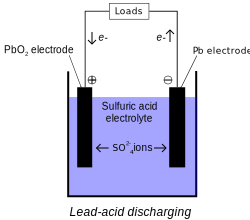
\includegraphics[height=5cm]{./images/Lead-acid_discharging.svg}$
	\end{multicols}
\end{flashcard}

























\end{document}
